\documentclass{ieeeaccess}
\usepackage{cite}
\usepackage{amsmath,amssymb,amsfonts}
\usepackage{algorithmic}
\usepackage{graphicx}
\usepackage{textcomp}
\usepackage{booktabs}
\usepackage{url}

\graphicspath{{figures/}}

% ── Paper macros ─────────────────────────────────────────────────────────
\newcommand{\arr}{\mathrm{ARR}}
\newcommand{\frr}{\mathrm{FRR}}
\newcommand{\aurc}{\mathrm{AURC}}
\newcommand{\clip}{\textsc{CLIP}}
\newcommand{\dinov}{\textsc{DINOv2}}
\newcommand{\mobilenet}{\textsc{MobileNetV3}}
\newcommand{\vilt}{\textsc{ViLT}}

\def\BibTeX{{\rm B\kern-.05em{\sc i\kern-.025em b}\kern-.08em
    T\kern-.1667em\lower.7ex\hbox{E}\kern-.125emX}}

\begin{document}

\history{Date of publication xxxx 00, 0000, date of current version xxxx 00, 0000.}
\doi{10.1109/ACCESS.2026.DOI}

\title{Knowing When and Why to Refuse: Defect-Aware Explanation and Recovery for Assistive Visual Question Answering}

% TODO: replace author metadata, affiliations, and funding before submission.
\author{\uppercase{First A. Author}\authorrefmark{1}}
\address[1]{Department, University, City, Country (e-mail: author@example.com)}
\tfootnote{}

\markboth
{Author \headeretal: Knowing When and Why to Refuse: Defect-Aware Explanation and Recovery for Assistive VQA}
{Author \headeretal: Knowing When and Why to Refuse: Defect-Aware Explanation and Recovery for Assistive VQA}

\corresp{Corresponding author: First A. Author (e-mail: author@example.com).}

\begin{abstract}
Visual question answering (VQA) systems for blind and low-vision users must do more than return an answer: they must know when an answer is unreliable, explain why the interaction failed, and help the user recover. This article studies a lightweight reliability layer for assistive VQA that combines answerability triage, human-labeled image-quality defect diagnosis, selective-prediction diagnostics, and actionable retake guidance. Using VizWiz-VQA and VizWiz-QualityIssues, real answerability labels are joined with seven human-annotated quality defects: blur, brightness, darkness, obstruction, framing, rotation, and unrecognizable content. Small prediction heads trained on frozen CLIP, DINOv2, and MobileNetV3 embeddings estimate answerability and defects, while a frozen ViLT model provides the answer and its confidence. The strongest triage head reaches an area under the receiver operating characteristic curve of 0.7926 with CLIP; the strongest defect head reaches a mean average precision of 0.6309 with DINOv2; and the best actionable recovery rate is 0.7196 with CLIP. However, defect-aware risk scores do not significantly reduce the area under the risk-coverage curve relative to the VQA model's own confidence, and adding even ground-truth defect labels to a learned confidence-based risk model slightly degrades it. Defect diagnosis is therefore best viewed not as a replacement for confidence-based risk ranking, but as an interpretable refusal-and-recovery mechanism: confidence indicates whether to trust an answer, while defect diagnosis explains why the system refuses and tells the user what to do next.
\end{abstract}

\begin{keywords}
Accessibility, assistive technology, calibration, image quality assessment, selective prediction, visual question answering.
\end{keywords}

\titlepgskip=-15pt

\maketitle

\section{Introduction}
\label{sec:introduction}
\PARstart{V}{isual} question answering (VQA) has become a natural interface for assistive technology: a blind or low-vision user can capture an image, ask a question, and receive a textual answer. Yet this setting is also unusually fragile. Images are captured in uncontrolled conditions, often without visual feedback, and the content needed to answer the question may be blurred, poorly framed, occluded, overexposed, underexposed, rotated, or impossible to recognize. The VizWiz benchmark was created precisely to reflect this real-world setting: its questions originate from blind users and frequently cannot be answered from the submitted image \cite{gurari2018vizwiz}.

Reliability in assistive VQA is therefore not only a matter of answer accuracy. A system must decide when to abstain, but it should also explain why the image or question is not answerable and provide useful recovery advice. Existing reliable VQA work has largely framed this problem as selective prediction: answer when the model is likely correct and abstain otherwise \cite{whitehead2022reliable,dancette2023improving}. This framing is essential, but it does not directly tell a user how to fix the failed interaction. Separately, the VizWiz-QualityIssues dataset provides human annotations for real image-quality flaws in images captured by blind users \cite{chiu2020assessing}. These labels create an opportunity to connect abstention with explanation and recovery.

This article studies that connection. We build a lightweight reliability layer around a frozen VQA model. The layer predicts answerability and image-quality defects from frozen visual embeddings, harvests the VQA model's answer confidence, evaluates selective-prediction behavior, and maps predicted defects to retake guidance. Importantly, our experiments show a negative but useful result: defect-aware selective-prediction scores do not significantly improve risk-coverage ranking over the VQA model's own confidence, and even a learned risk model given ground-truth defect labels in addition to confidence performs slightly worse than confidence alone. This finding changes the role of defect diagnosis. Rather than replacing confidence as the risk-ranking signal, defect diagnosis provides interpretable refusal reasons and actionable recovery advice.

Our contributions are:
\begin{itemize}
    \item We join VizWiz-VQA answerability labels with VizWiz-QualityIssues defect labels to study answerability, quality diagnosis, and recovery in one assistive VQA pipeline.
    \item We train lightweight answerability and multi-label defect heads on frozen \clip{} \cite{radford2021clip}, \dinov{} \cite{oquab2023dinov2}, and \mobilenet{} \cite{howard2019mobilenetv3} embeddings, benchmarking modern visual backbones under identical evaluation conditions.
    \item We introduce the Actionable Recovery Rate ($\arr$) and False Refilm Rate ($\frr$) to evaluate whether predicted defects lead to useful retake guidance rather than merely abstention.
    \item We report a selective-prediction diagnostic: predicted defects, defect-conditioned calibration, and even ground-truth defects added to a learned confidence-based risk model do not improve the area under the risk-coverage curve ($\aurc$) over global VQA confidence in this setup. This supports a deployment design in which confidence ranks risk while defect diagnosis explains refusals and guides recovery.
\end{itemize}

\section{Related Work}
\label{sec:related}

\subsection{Assistive Visual Question Answering}
The VizWiz VQA dataset introduced a goal-oriented VQA benchmark whose images and spoken questions come from blind users \cite{gurari2018vizwiz,vizwizvqaweb}. Unlike many synthetic or curated VQA datasets, VizWiz contains conversational questions, low-quality images, and a substantial number of unanswerable examples. This makes it a natural testbed for reliability and refusal in assistive VQA.

\subsection{Image Quality in Real-World Assistive Images}
Chiu \emph{et al.} introduced VizWiz-QualityIssues, a dataset of image-quality annotations for images captured by blind users \cite{chiu2020assessing,vizwizqualityweb}. The labels include whether image content is recognizable and which flaws are present. Their work links image-quality assessment to practical vision tasks including captioning and VQA. Our article uses these human defect labels not only as an image-quality prediction task, but also as the basis for refusal explanation and retake guidance.

\subsection{Selective Prediction and Reliable VQA}
Selective prediction allows a model to answer only when it is sufficiently reliable, trading coverage against risk \cite{elyaniv2010foundations}. Reliable VQA work has applied this idea to VQA systems, showing that softmax confidence can be insufficient and that learned selection functions can improve abstention behavior \cite{whitehead2022reliable,dancette2023improving}. Recent work further studies selectively answering visual questions under uncertainty \cite{eisenschlos2024selectively}. Our experiments differ in focus: we test whether image-quality defect diagnosis improves selective prediction in assistive VQA and find that it does not outperform global VQA confidence for $\aurc$ in our setting.

\subsection{Frozen Visual and Vision-Language Models}
We evaluate frozen visual representations from \clip{} \cite{radford2021clip}, \dinov{} \cite{oquab2023dinov2}, and \mobilenet{} \cite{howard2019mobilenetv3}. We use \vilt{} \cite{kim2021vilt} as a frozen discriminative VQA model to harvest answer predictions and confidence scores. This design keeps the reliability layer lightweight and separates reliability evaluation from VQA model training.

\section{Data}
\label{sec:data}

\subsection{Datasets}
We use VizWiz-VQA \cite{gurari2018vizwiz} and VizWiz-QualityIssues \cite{chiu2020assessing}. VizWiz-VQA provides an image filename, a natural-language question, ten crowdsourced answers, answer-type metadata, and an answerability flag. VizWiz-QualityIssues provides image-level quality labels: blur, bright, dark, obstruction, framing, rotation, and unrecognizable content. Each image was labeled by five crowdworkers; following the dataset authors, a label is considered present when at least two crowdworkers selected it \cite{chiu2020assessing}.

\subsection{Joining Labels}
The two datasets are joined by image filename and split. We keep examples that have both VQA answerability labels and quality-issue labels. In the current run this produces 24{,}319 rows: 20{,}000 training rows and 4{,}319 validation rows. Validation is further split into a calibration subset and a report subset. All thresholds, temperatures, and learned risk-score models are fit on calibration data only; all reported selective-prediction metrics are computed on the report subset.

\subsection{Label Distribution}
The answerable rate after joining is 0.7214. Quality labels are highly imbalanced. Framing and blur are the most common defects, with positive rates 0.5606 and 0.4161, respectively. Bright, dark, and obstruction are much rarer, with positive rates 0.0539, 0.0563, and 0.0352. These imbalances motivate per-defect reporting and caution against relying on accuracy alone. Figure~\ref{fig:label_distribution} summarizes the label structure.

\begin{figure}[t]
    \centering
    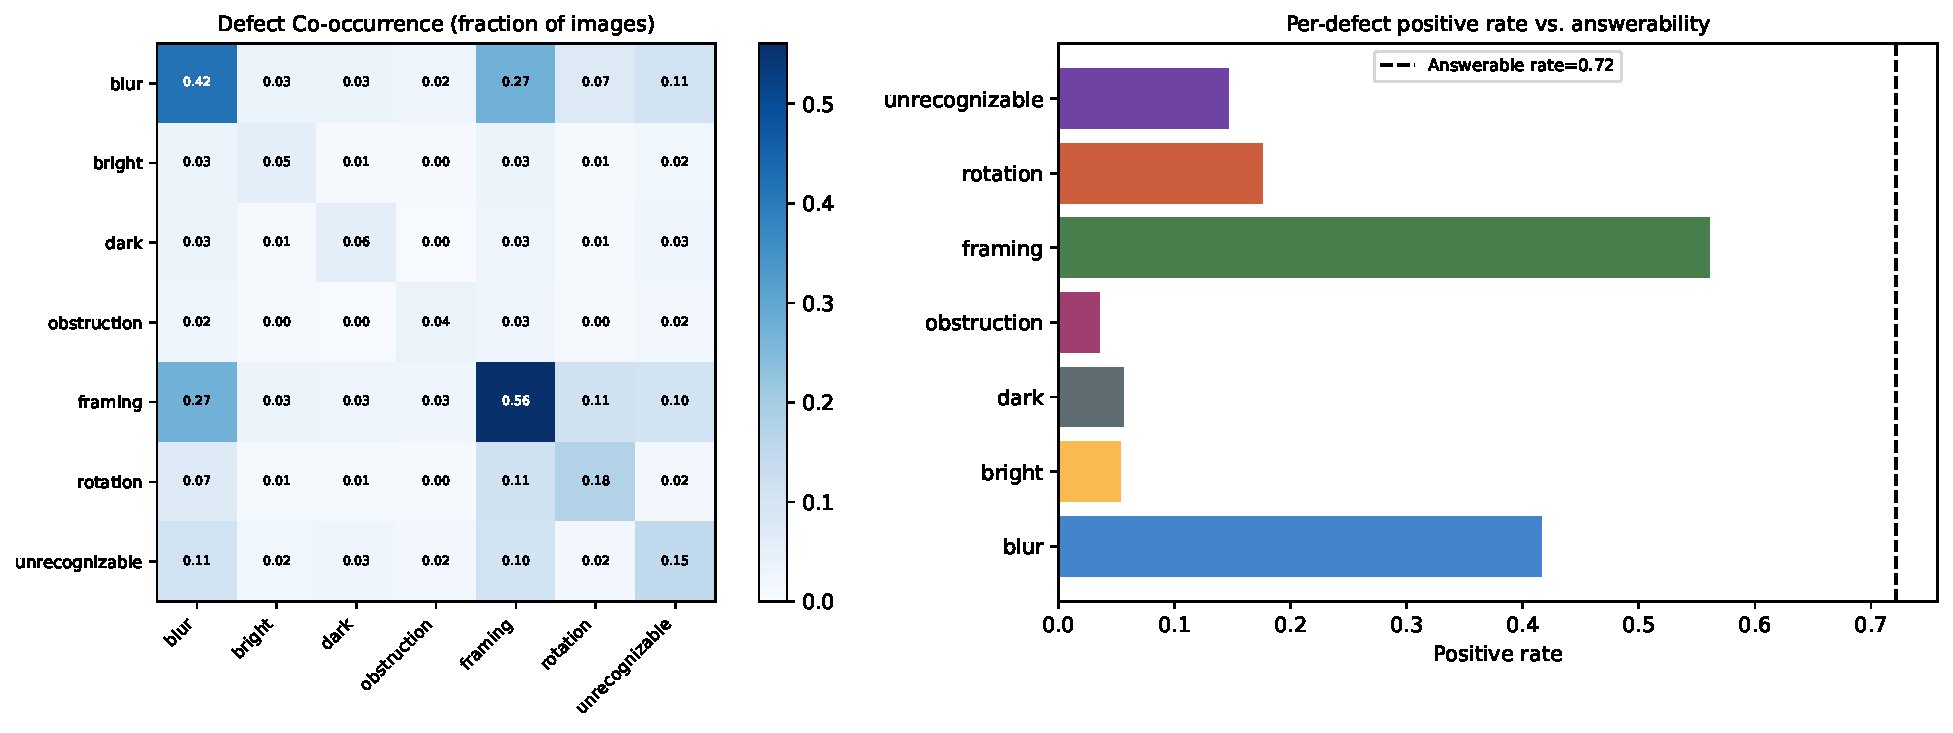
\includegraphics[width=\linewidth]{F2_cooccurrence.pdf}
    \caption{Quality-label structure in the joined data. The left panel shows pairwise defect co-occurrence, while the right panel shows per-defect prevalence relative to the answerable rate. The skewed distribution motivates per-defect metrics and recovery analysis rather than aggregate accuracy alone.}
    \label{fig:label_distribution}
\end{figure}

\section{Method}
\label{sec:method}

Figure~\ref{fig:pipeline} summarizes the pipeline. A frozen image encoder produces visual embeddings. Lightweight heads predict answerability and quality defects. Separately, a frozen VQA model answers the question and emits confidence. The system can then decide whether to answer, refuse, and provide retake guidance.

\begin{figure}[t]
    \centering
    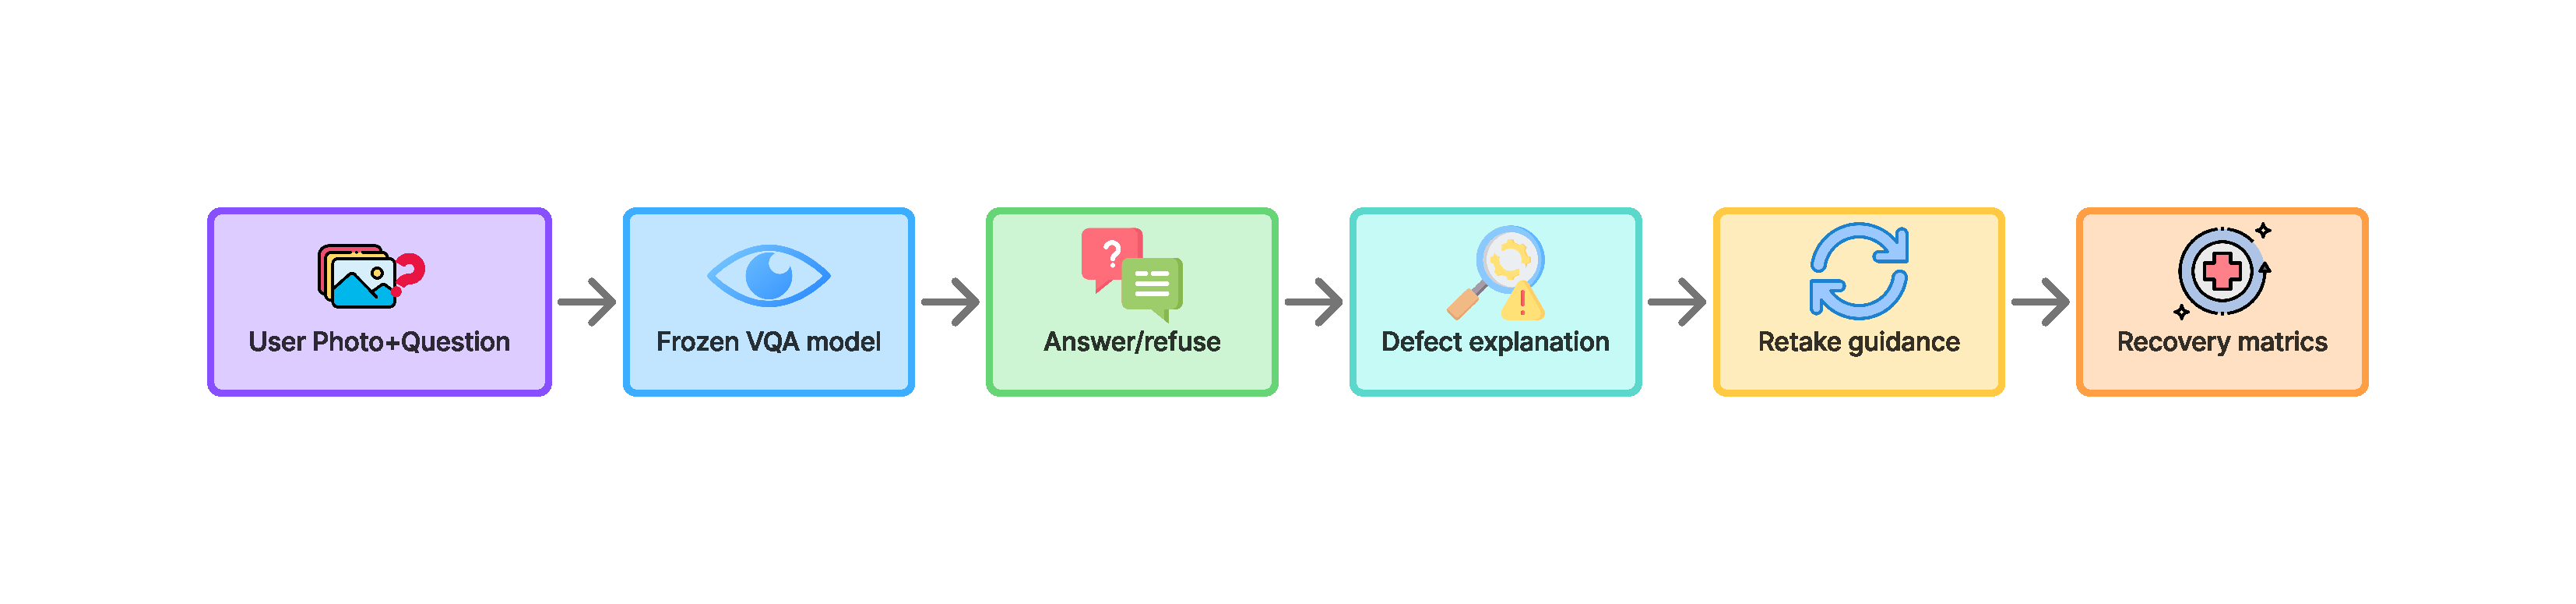
\includegraphics[width=\linewidth]{F1_pipeline_schematic.pdf}
    \caption{Overview of the reliability layer. Frozen visual features feed answerability and defect heads. Frozen VQA confidence provides the main risk-ranking signal. Predicted defects provide refusal explanation and retake guidance.}
    \label{fig:pipeline}
\end{figure}

\subsection{Frozen Backbones}
We compare three frozen image encoders: \clip{} ViT-B/32, \dinov{} ViT-S/14, and \mobilenet-Large. The resulting embeddings are cached once and reused by all downstream heads. This keeps the experiments reproducible and avoids recomputing expensive features.

\subsection{Answerability Triage}
For each backbone, a small multilayer perceptron predicts the VizWiz answerability label. Heads are trained on the training split with five random seeds; thresholds are selected on the calibration split, and final metrics are reported on the held-out report split as the mean and standard deviation over seeds.

\subsection{Defect Diagnosis}
The defect head is a multi-label classifier over seven labels: blur, bright, dark, obstruction, framing, rotation, and unrecognizable. Each label is evaluated one-vs-rest, and macro/micro summaries are reported alongside per-defect AUROC and AUPRC.

\subsection{Frozen VQA Confidence}
We use a frozen \vilt{} model fine-tuned for VQA to obtain a predicted answer and a maximum-softmax confidence for each example. VizWiz answer accuracy is computed as $\min(m/3, 1)$, where $m$ is the number of exact matches between the predicted answer and the ten human answers.

\subsection{Recovery Mapping}
Each predicted defect maps to a fixed user-facing retake action. For example, blur maps to holding the camera steady and refocusing, dark maps to adding light, and framing maps to stepping back so the full object is visible. This deterministic mapping is used to evaluate actionable recovery.

\section{Evaluation Metrics}
\label{sec:metrics}

\subsection{Answerability and Defect Prediction}
Answerability triage is evaluated using AUROC, AUPRC, F1, balanced accuracy, and a majority-class baseline. Defect diagnosis is evaluated as a multi-label problem using per-defect AUROC and AUPRC, macro-F1, micro-F1, and mean average precision (mAP).

\subsection{Selective Prediction}
Selective prediction is evaluated with risk-coverage curves and the area under the risk-coverage curve ($\aurc$) \cite{elyaniv2010foundations}. Lower $\aurc$ indicates a better risk ranking. We compare global VQA confidence, temperature-scaled confidence \cite{guo2017calibration}, defect-conditioned calibration, learned risk scores that combine confidence with predicted defects, and a learned risk score that combines confidence with ground-truth defects (an oracle upper bound on defect information). Statistical comparisons use paired bootstrap confidence intervals on the report split.

\subsection{Actionable Recovery}
We define the Actionable Recovery Rate ($\arr$) as the fraction of unanswerable examples for which the predicted defect leads to a corrective action matching a ground-truth defect. Concretely, the system selects the top-scoring predicted defect if its probability exceeds 0.5; the example counts as a recovery hit if that defect is present in the ground truth, and as a miss if no defect is predicted or the top prediction is wrong. We define the False Refilm Rate ($\frr$) as the fraction of answerable examples for which the system would suggest a retake, i.e., predicts any defect above threshold. $\arr$ rewards useful recovery guidance; $\frr$ measures potential user burden. Note that $\frr$ is a conservative burden proxy: many answerable VizWiz images genuinely contain defects, so a truthful defect prediction on an answerable image still counts against $\frr$. In deployment, retake guidance would additionally be gated by the answer/refuse decision.

\subsection{Joint Versus Cascade}
To quantify architecture effects, we compare a cascade design with separate answerability and defect heads against a joint multi-task head. We report the change in answerability AUROC between joint and cascade designs.

\section{Results}
\label{sec:results}

\subsection{Data Sanity}
The joined dataset contains 24{,}319 rows, with 20{,}000 training examples and 4{,}319 validation examples. The frozen \vilt{} model obtains mean VizWiz answer accuracy 0.1853 and mean confidence 0.4469, confirming that the downstream reliability problem is challenging.

\subsection{Answerability Triage}
\clip{} performs best for answerability triage, reaching AUROC $0.7926 \pm 0.0005$ and AUPRC $0.8811$. \dinov{} reaches AUROC $0.7769 \pm 0.0005$, while \mobilenet{} reaches AUROC $0.7512 \pm 0.0009$. All three exceed the majority-class F1 baseline of 0.809 (model F1 0.823--0.836), although the margins are modest; balanced accuracy (0.59--0.66) gives a more conservative picture of triage quality. Table~\ref{tab:core_results} and Figure~\ref{fig:backbone_comparison} summarize the comparison.

\begin{figure}[t]
    \centering
    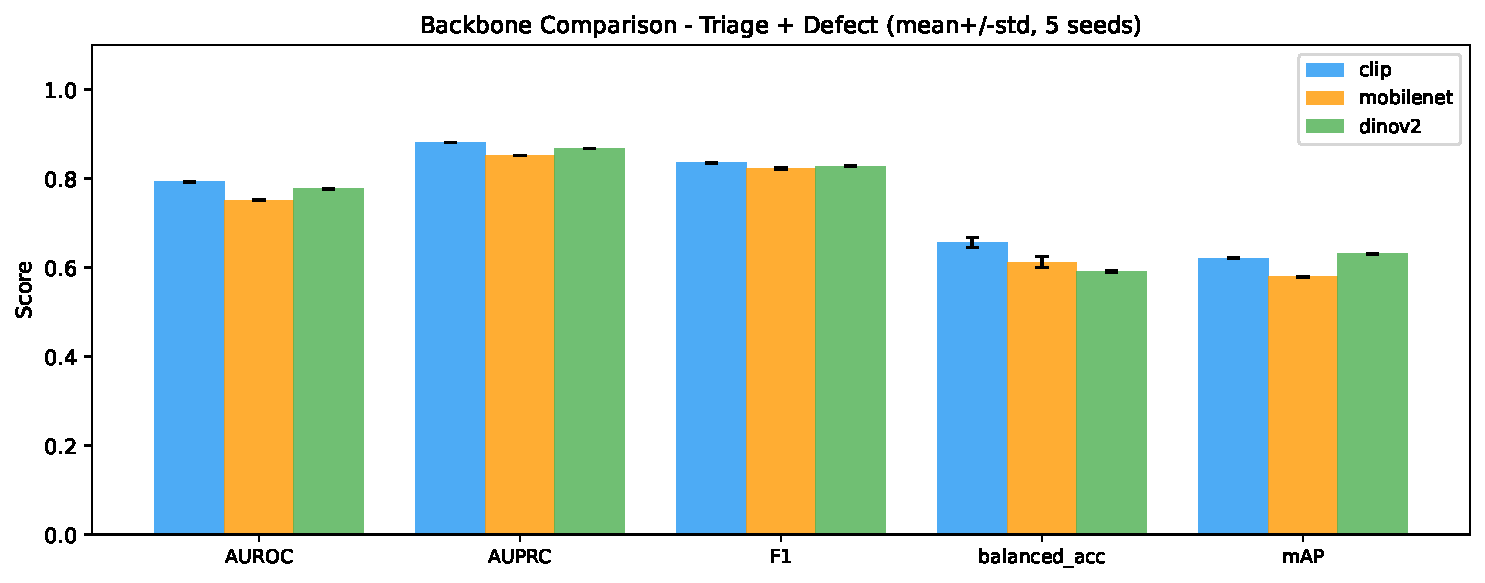
\includegraphics[width=\linewidth]{F7_backbone_comparison.pdf}
    \caption{Backbone comparison for answerability triage and multi-label defect diagnosis. \clip{} is strongest for answerability triage, while \dinov{} gives the highest defect mAP. Error bars show variation over five random seeds.}
    \label{fig:backbone_comparison}
\end{figure}

\subsection{Defect Diagnosis}
\dinov{} provides the strongest defect diagnosis by mAP, reaching $0.6309 \pm 0.0009$. \clip{} follows at $0.6216 \pm 0.0007$, and \mobilenet{} reaches $0.5801 \pm 0.0011$. Across backbones, unrecognizable content is the easiest defect to identify (AUROC 0.93 with \clip), while framing is the hardest by AUROC (0.83). Under AUPRC, the rare defects---obstruction, bright, and dark---drop sharply (0.33--0.48), exposing the effect of class imbalance. Figure~\ref{fig:per_defect} shows the per-defect breakdown.

\begin{figure*}[t]
    \centering
    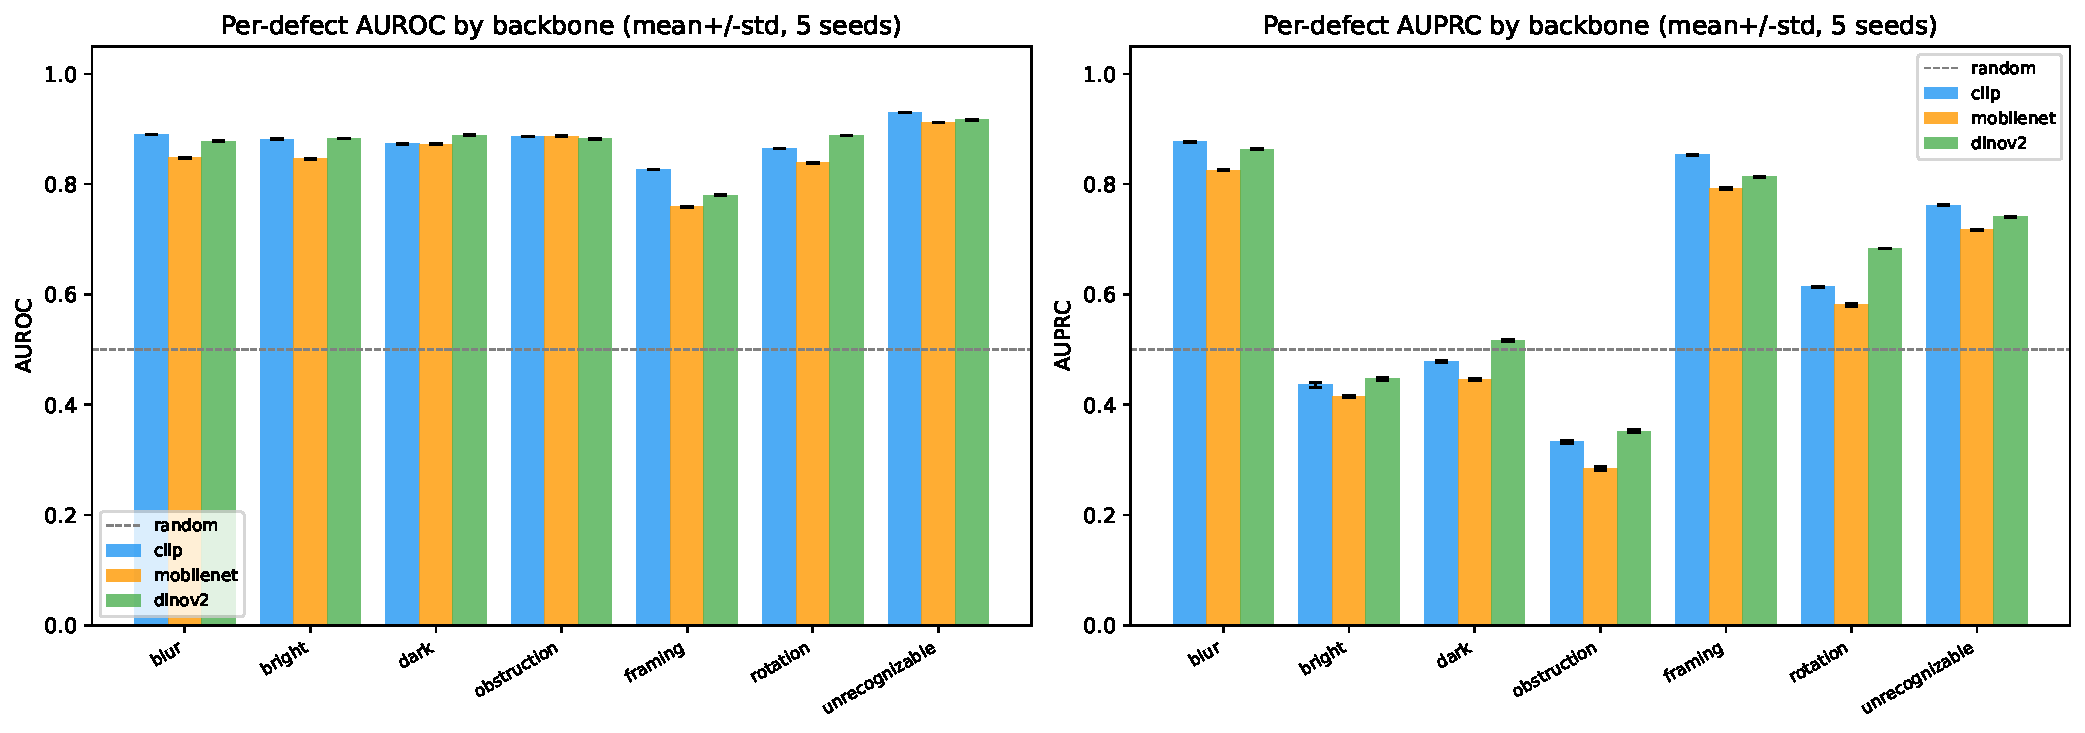
\includegraphics[width=0.92\textwidth]{F3_per_defect_auroc_auprc.pdf}
    \caption{Per-defect diagnosis performance by backbone. AUROC is high for most defects, with framing the hardest label by AUROC. AUPRC exposes the effect of class imbalance: the rare defects (obstruction, bright, and dark) score far lower under AUPRC despite high AUROC.}
    \label{fig:per_defect}
\end{figure*}

\begin{table*}[t]
    \centering
    \caption{Core reliability-layer results. Triage AUROC and defect mAP are mean $\pm$ standard deviation over five seeds; $\arr$/$\frr$ show bootstrap 95\% confidence intervals.}
    \label{tab:core_results}
    \begin{tabular}{lcccccc}
        \toprule
        Backbone & Triage AUROC & Triage AUPRC & Defect mAP & $\arr$ [95\% CI] & $\frr$ [95\% CI] & Joint$-$Cascade $\Delta$AUROC \\
        \midrule
        \clip{}      & $0.7926 \pm 0.0005$ & 0.8811 & $0.6216 \pm 0.0007$ & 0.7196 [0.692, 0.750] & 0.7746 [0.756, 0.793] & $+0.0013$ \\
        \dinov{}     & $0.7769 \pm 0.0005$ & 0.8676 & $0.6309 \pm 0.0009$ & 0.6907 [0.660, 0.719] & 0.7775 [0.760, 0.796] & $+0.0028$ \\
        \mobilenet{} & $0.7512 \pm 0.0009$ & 0.8524 & $0.5801 \pm 0.0011$ & 0.6278 [0.597, 0.658] & 0.7780 [0.760, 0.795] & $+0.0037$ \\
        \bottomrule
    \end{tabular}
\end{table*}

\subsection{Actionable Recovery}
\clip{} obtains the highest actionable recovery rate, $\arr$ 0.7196, followed by \dinov{} at 0.6907 and \mobilenet{} at 0.6278. All methods have high false refilm rates near 0.78. As noted in Section~\ref{sec:metrics}, this partly reflects the genuine prevalence of defects among answerable images (framing alone affects 56\% of images); nevertheless, it indicates that a deployed system should issue retake guidance only after the answer/refuse decision and should tune recovery policies with user burden in mind. Figure~\ref{fig:arr_frr} breaks recovery down by defect type.

\begin{figure}[t]
    \centering
    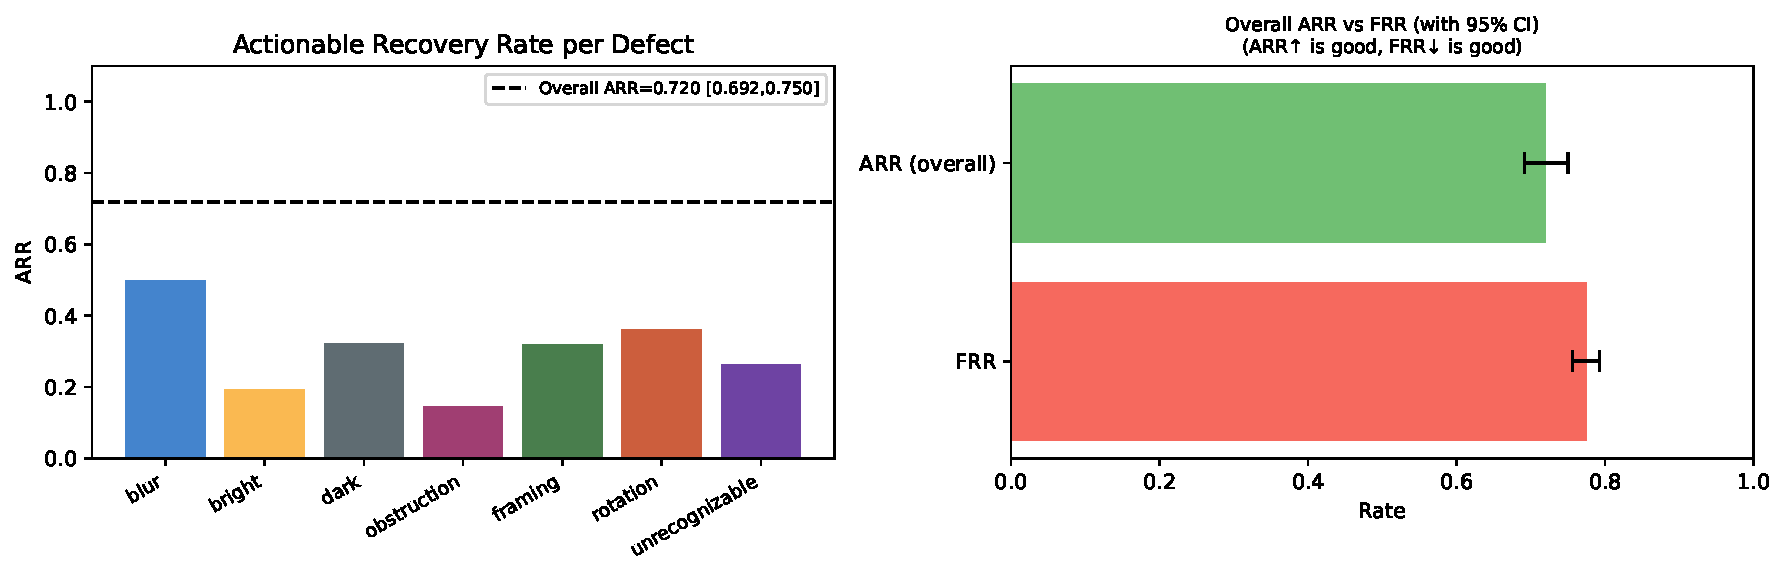
\includegraphics[width=\linewidth]{F6_arr_frr.pdf}
    \caption{Actionable recovery from predicted defects. The left panel breaks down recovery by defect type; the right panel contrasts overall actionable recovery against the false refilm rate. The high false refilm rate underscores the need for cost-sensitive, refusal-gated recovery policies.}
    \label{fig:arr_frr}
\end{figure}

\subsection{Selective Prediction}
The original hypothesis was that defect-aware risk scores would improve selective prediction over global VQA confidence. The experiments do not support this. Global VQA confidence achieves $\aurc$ 0.5357 on the report split (a random ordering yields 0.7460). Temperature scaling \cite{guo2017calibration} fitted on the calibration split leaves the ranking unchanged ($\aurc$ identical, as expected for a monotone transform) and slightly worsens the expected calibration error on the report split (0.194 raw versus 0.202 scaled). Defect-conditioned calibration produces small and statistically unsupported $\aurc$ changes ($p \geq 0.30$ across backbones). A learned risk model combining confidence with predicted-defect features is also statistically unsupported ($p \geq 0.42$). Most strikingly, a learned risk model given \emph{ground-truth} defect labels in addition to confidence performs slightly but significantly \emph{worse} than confidence alone (improvement $-0.0053$, 95\% CI $[-0.0107, -0.0003]$, $p = 0.039$): the added defect features do not carry usable ranking signal beyond confidence, and fitting them on the calibration split degrades generalization to the report split. Figure~\ref{fig:calibration_risk}, Figure~\ref{fig:selective_diagnostic}, and Table~\ref{tab:selective} summarize these diagnostics.

\begin{figure*}[t]
    \centering
    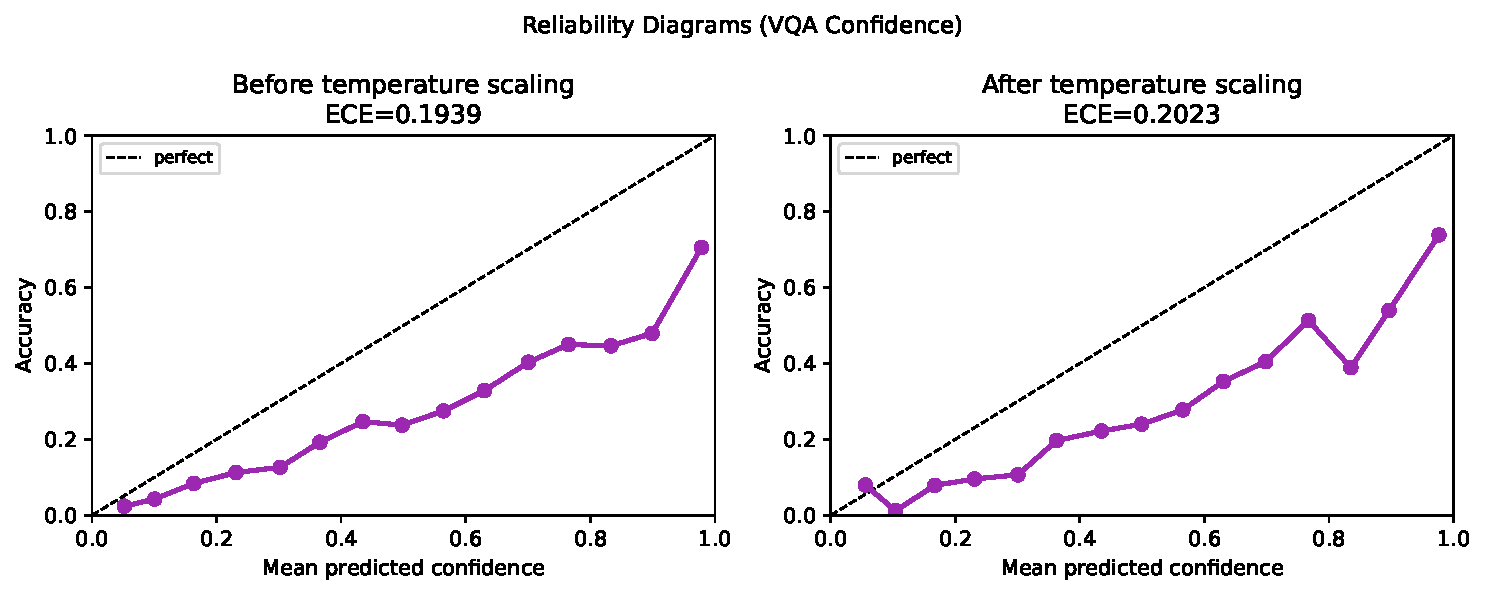
\includegraphics[width=0.48\textwidth]{F4_reliability_diagram.pdf}
    \hfill
    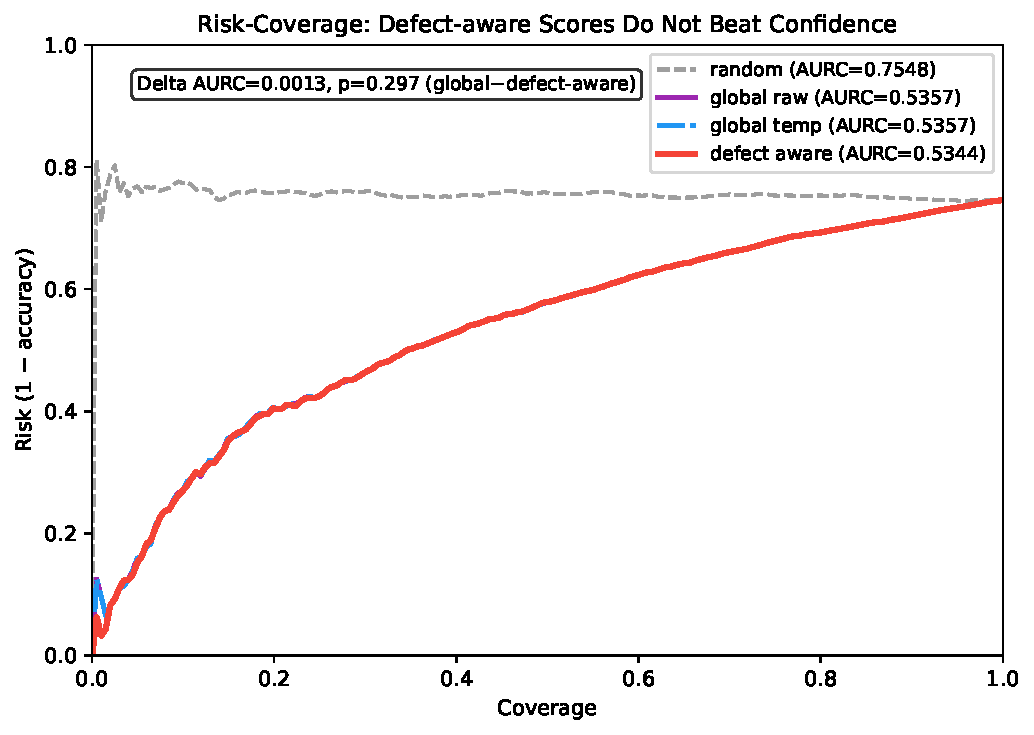
\includegraphics[width=0.48\textwidth]{F5_risk_coverage.pdf}
    \caption{Calibration and selective-prediction behavior for frozen VQA confidence. Temperature scaling does not close the reliability gap, and defect-aware risk scores do not improve the risk-coverage curve over global confidence.}
    \label{fig:calibration_risk}
\end{figure*}

\begin{figure}[t]
    \centering
    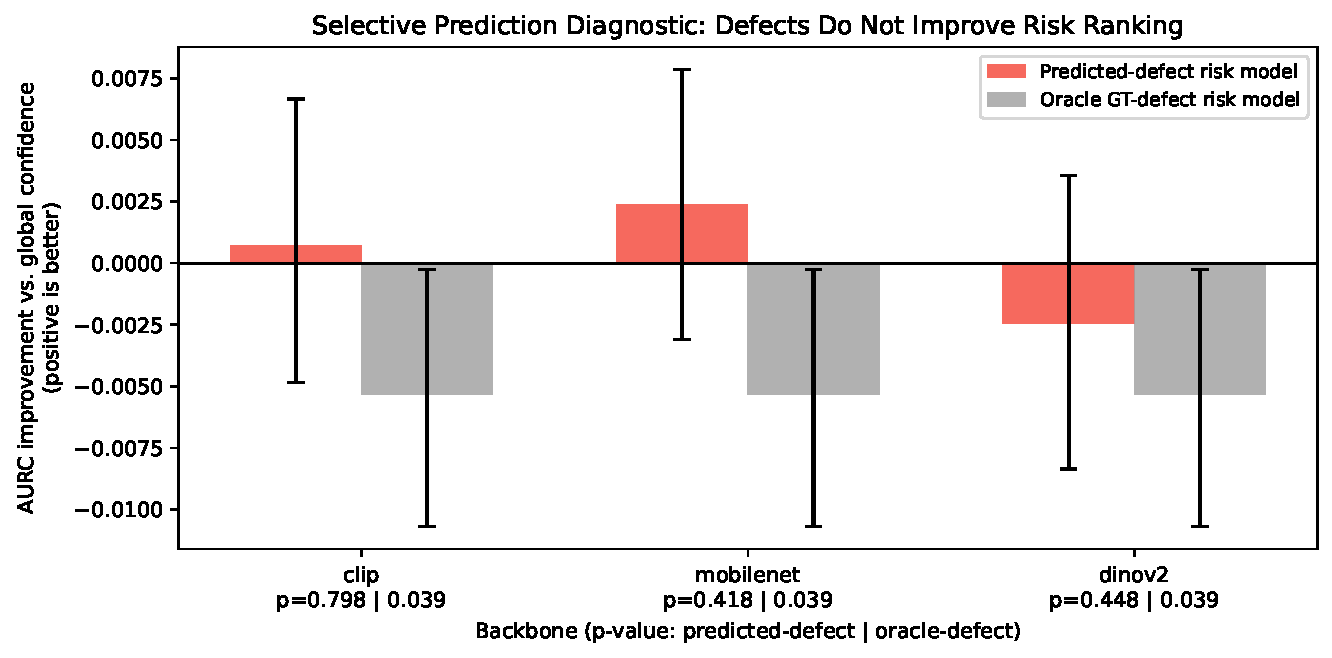
\includegraphics[width=\linewidth]{F8_selective_diagnostics.pdf}
    \caption{Selective-prediction diagnostics. Positive values indicate lower $\aurc$ than global VQA confidence. Risk models using predicted defects are not statistically supported, and adding ground-truth defects to a confidence-based risk model slightly degrades risk ranking.}
    \label{fig:selective_diagnostic}
\end{figure}

\begin{table*}[t]
    \centering
    \caption{Selective-prediction diagnostics on the report split. Positive improvement means lower $\aurc$ than global VQA confidence ($\aurc$ 0.5357; random ordering 0.7460). The oracle model uses confidence plus ground-truth defects and is therefore backbone-independent; it is reported once.}
    \label{tab:selective}
    \begin{tabular}{lcc}
        \toprule
        Method & $\aurc$ improvement & $p$ \\
        \midrule
        Defect-conditioned calibration (\clip)      & $+0.0009$ & 0.297 \\
        Defect-conditioned calibration (\dinov)     & $-0.0001$ & 0.923 \\
        Defect-conditioned calibration (\mobilenet) & $+0.0008$ & 0.361 \\
        \midrule
        Learned risk: confidence + predicted defects (\clip)      & $+0.0007$ & 0.798 \\
        Learned risk: confidence + predicted defects (\dinov)     & $-0.0024$ & 0.448 \\
        Learned risk: confidence + predicted defects (\mobilenet) & $+0.0024$ & 0.418 \\
        \midrule
        Learned risk: confidence + ground-truth defects (oracle) & $-0.0053$ & 0.039 \\
        \bottomrule
    \end{tabular}
\end{table*}

\subsection{Joint Versus Cascade}
The joint head gives small but consistent AUROC gains over the cascade design: $+0.0013$ for \clip{}, $+0.0028$ for \dinov{}, and $+0.0037$ for \mobilenet{}. These gains are modest, suggesting that the choice of backbone matters more than the head architecture.

\section{Discussion}
\label{sec:discussion}

The results suggest a separation of roles. Among the signals we evaluated, VQA confidence is the strongest for ranking answer risk, while defect diagnosis is useful for explanation and recovery. This is plausible: a VQA model's confidence may already encode image quality, question difficulty, answer ambiguity, and model uncertainty in a single scalar. Image-quality defects are semantically meaningful, but they do not further order examples by VQA correctness once confidence is available.

This negative result should not be hidden. In assistive settings, an honest reliability layer should distinguish between knowing that an answer is risky and knowing why the interaction failed. A high-confidence answer may be returned directly. A low-confidence answer may be refused. When refusing, the defect head can explain the likely visual cause and suggest a retake action. This design avoids overstating what defect labels can do for calibration while preserving their user-facing value.

The high false refilm rates indicate that recovery policies should be cost-sensitive. Asking a blind or low-vision user to retake an image has a real usability cost. Future systems should issue retake guidance only after the refusal decision and tune recovery thresholds to balance helpful guidance against unnecessary burden.

\section{Limitations}
\label{sec:limitations}

This study uses VizWiz train and validation labels; hidden test answers are not evaluated. The frozen VQA model is \vilt, which obtains low absolute accuracy on the joined data, so results may differ with stronger modern vision-language models. The selective-prediction comparison covers defect-derived signals; other auxiliary risk signals could behave differently. $\arr$ and $\frr$ depend on a deterministic defect-to-action map that should eventually be validated with users, and $\frr$ counts truthful defect predictions on answerable images as burden. Quality defects explain many image failures but not all reasons a VQA answer can be wrong, such as semantic ambiguity, text-reading failures, or missing world knowledge. Finally, spatial grounding is not included in the core results; it remains future work.

\section{Conclusion}
\label{sec:conclusion}

We studied a defect-aware reliability layer for assistive VQA using real answerability and image-quality labels from VizWiz. Lightweight heads on frozen visual backbones can predict answerability and diagnose visual defects, and these predictions support actionable retake guidance. At the same time, defect-aware risk scores do not outperform global VQA confidence for selective prediction, and even ground-truth defects add no usable ranking signal beyond confidence. The resulting lesson is practical: confidence should remain the primary risk-ranking signal, while defect diagnosis should be used to explain refusal and guide recovery.

\bibliographystyle{IEEEtran}
\bibliography{references}

% TODO: replace biography with real author information and photo before submission.
\begin{IEEEbiography}[{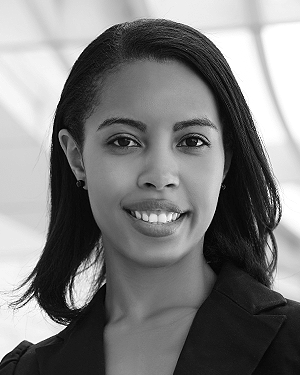
\includegraphics[width=1in,height=1.25in,clip,keepaspectratio]{a1.png}}]{First A. Author}
Biography text here. Replace with the author's education, experience, and research interests.
\end{IEEEbiography}

\EOD

\end{document}
